\chapter{Status}
\section{Linearity}
\subsection{Vertical displacement}
Measuring system is composed by an interferometer measuring BPM vertical position. As the head is located over the BPM, positive displacement implies negative change in the intereferometer lecture.\par
\begin{figure}[htb]
\begin{center}
\includegraphics[angle=180,scale=0.4]{interfero.jpg}\caption{Picture of SIOS interferometer used to test the movers. Precision is below 1nm.}\label{f-interfero}
\end{center}
\end{figure}\par
Test consist in 4 cycles, two descending and two rising over the total range divided in 100 steps. Time between steps is 3s.\par
\begin{figure}[htb]
\begin{center}
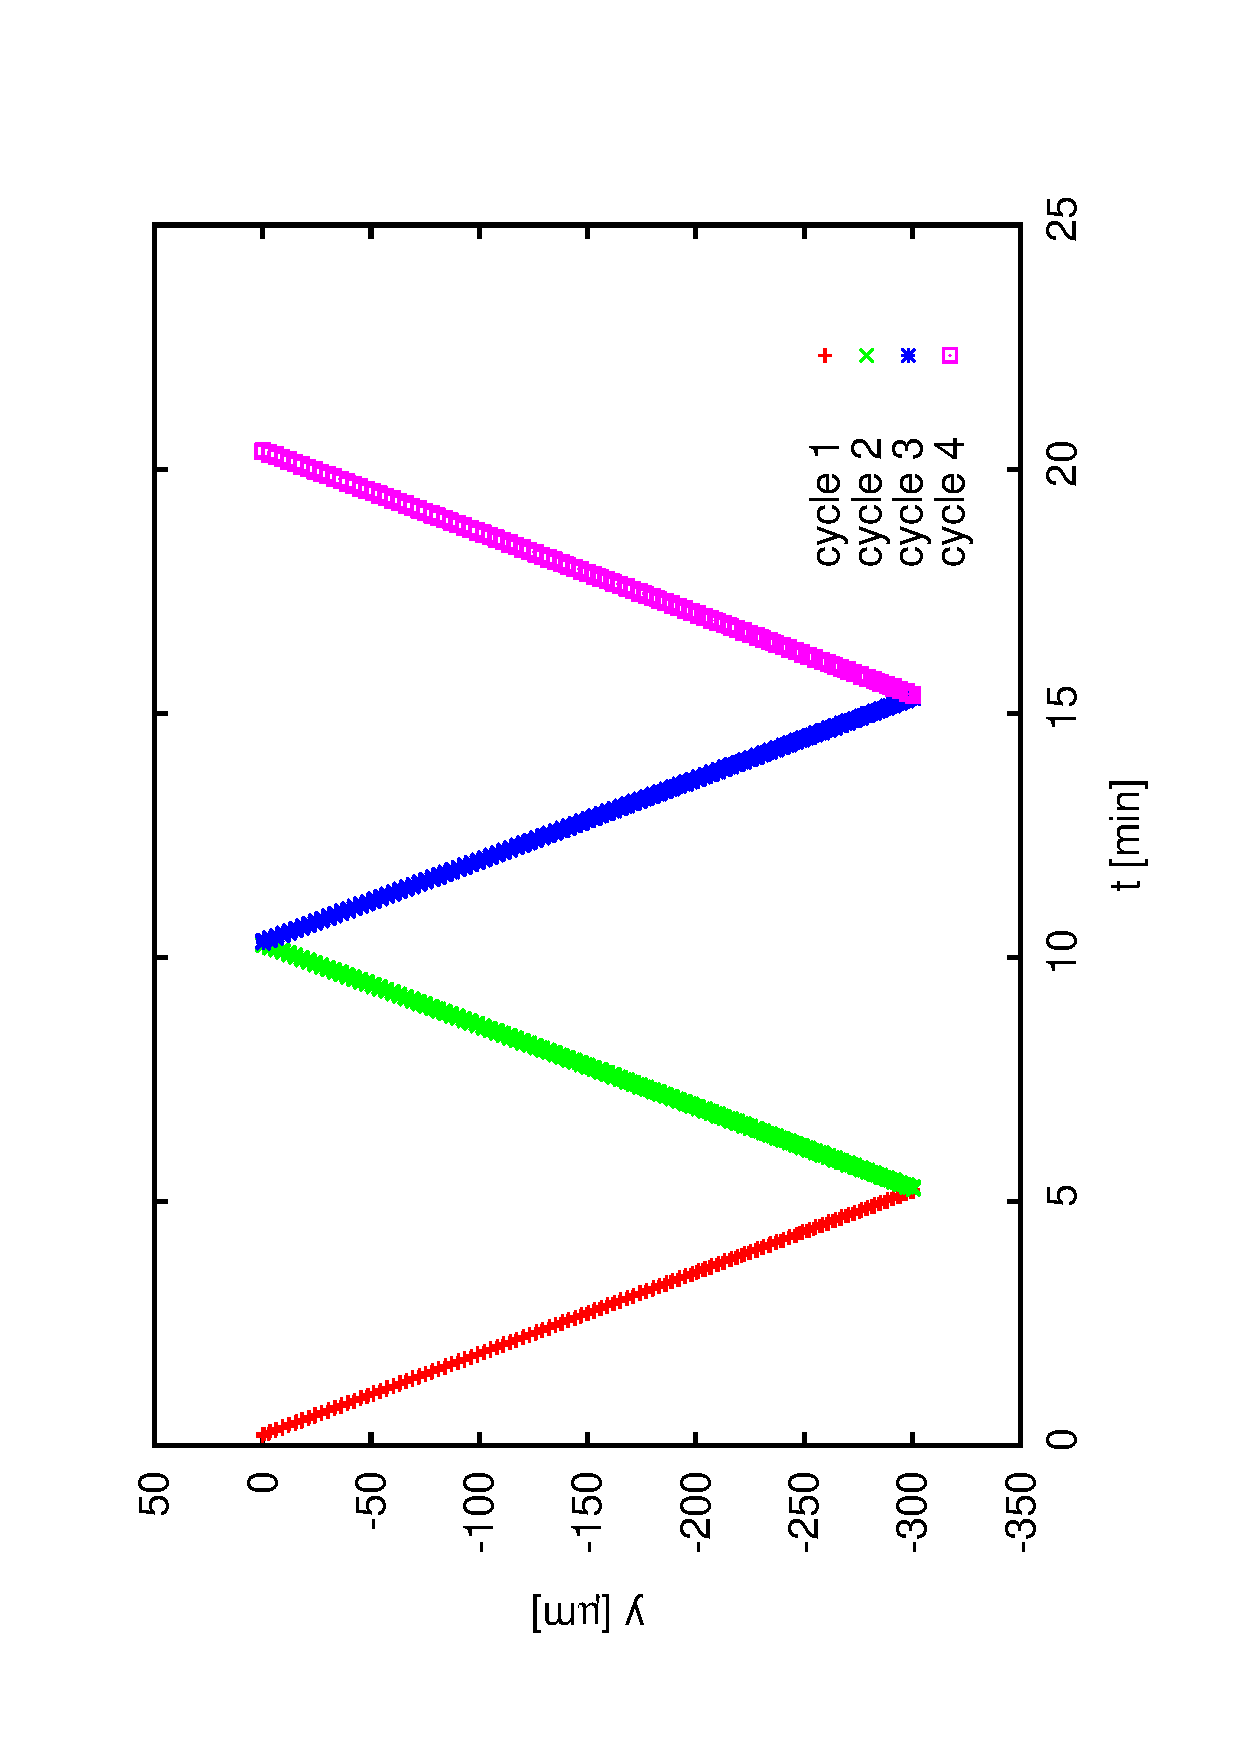
\includegraphics[scale=0.3,angle=-90]{image01.pdf}\caption{PI movers linearity.}\label{f-LinPI01}
\end{center}
\end{figure}
\subsubsection{PI without and with feedback}
Four cycles (two going up, two going down),
range (0$\sim$10V, 0$\sim$300$\mu$m)\par
\begin{figure}
 \begin{center}
\includegraphics[angle=-90,scale=0.20]{image11.pdf}
\includegraphics[angle=-90,scale=0.20]{image12.pdf}
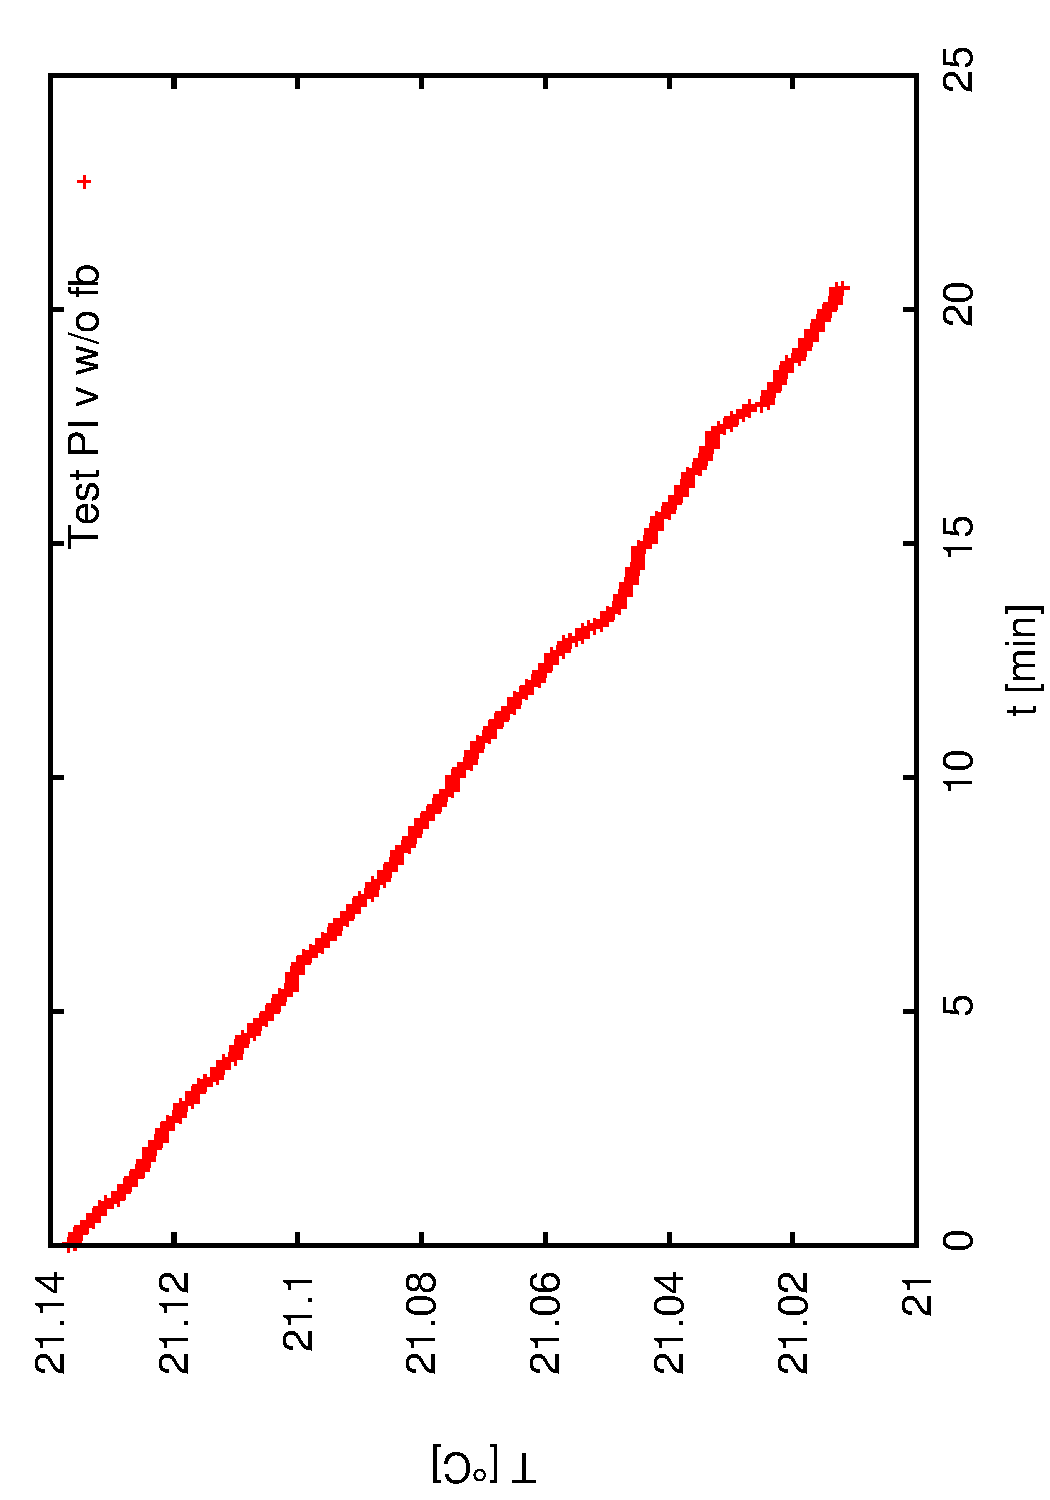
\includegraphics[angle=-90,scale=0.20]{image11a.pdf}\\
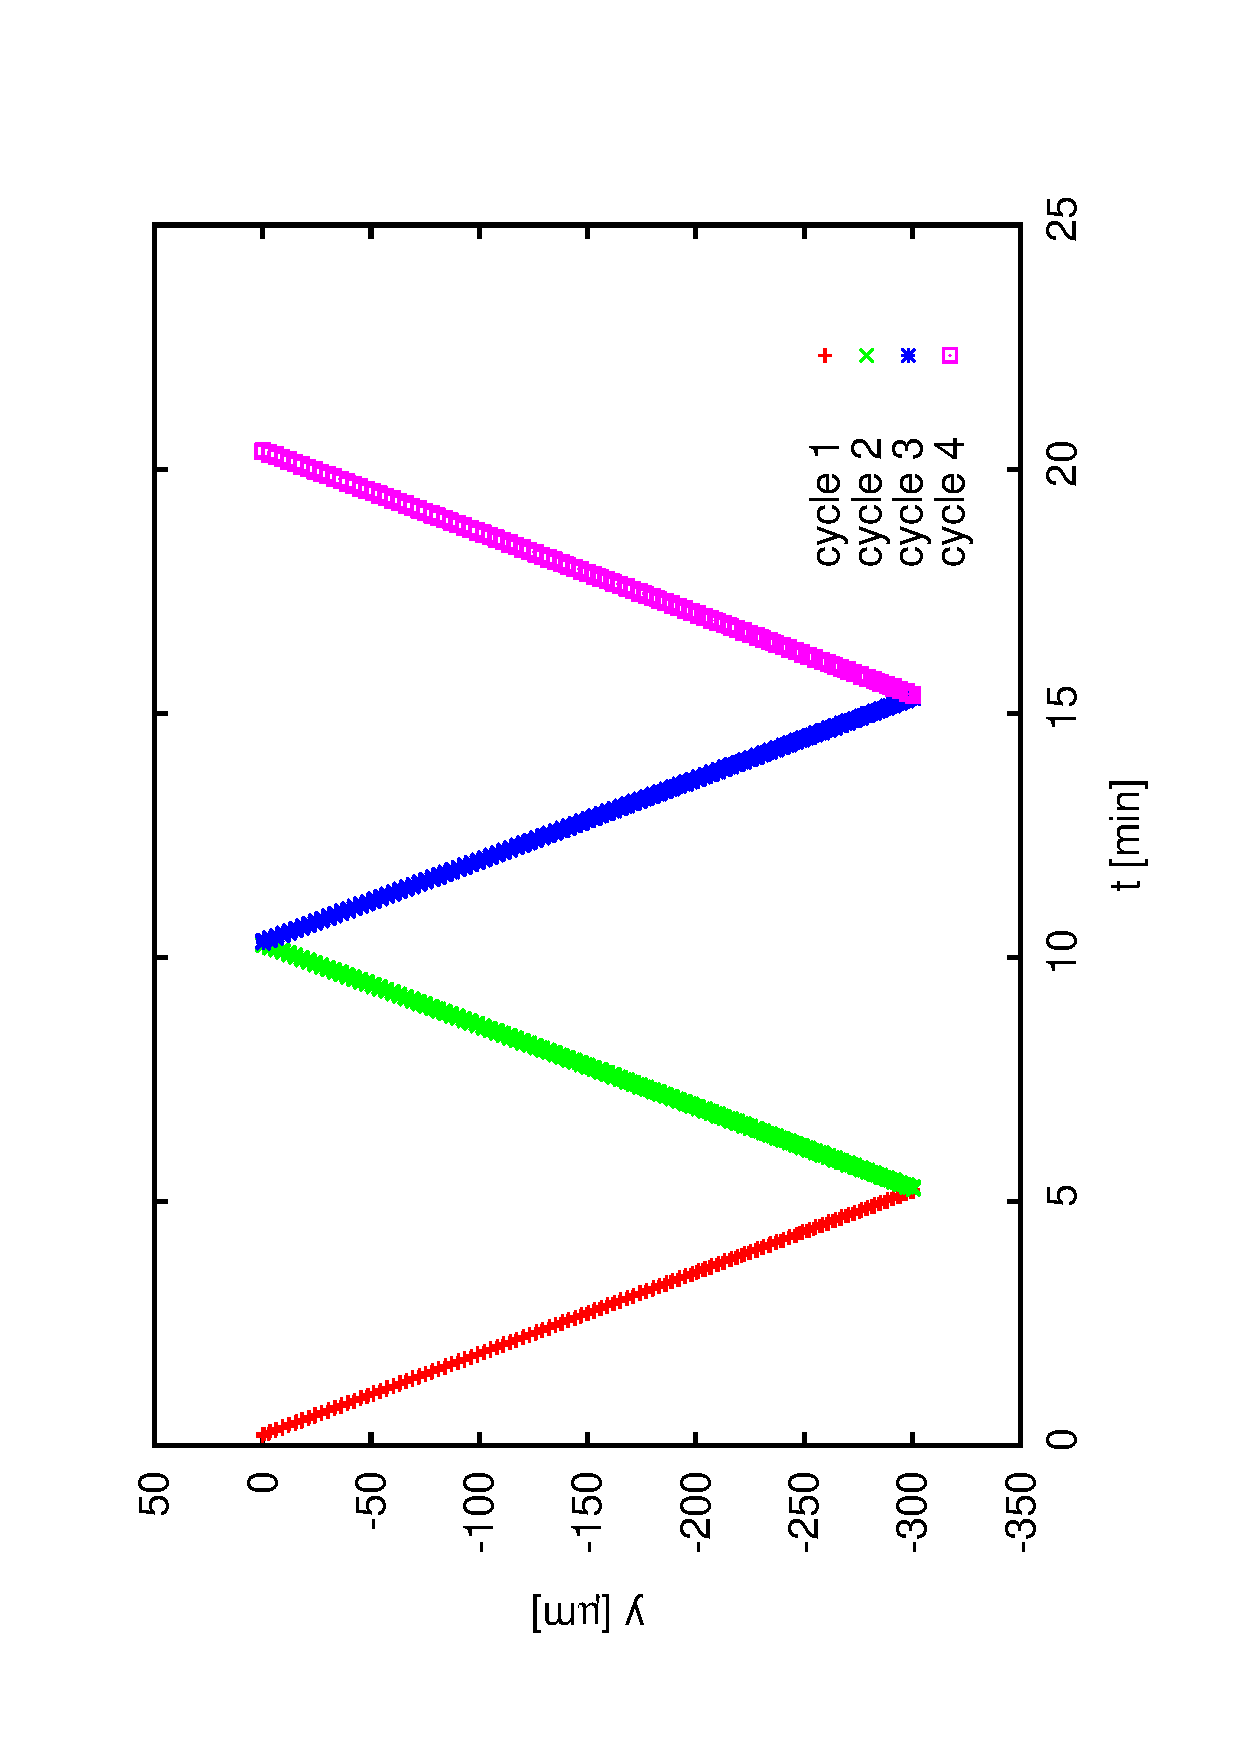
\includegraphics[angle=-90,scale=0.20]{image01.pdf}
\includegraphics[angle=-90,scale=0.20]{image02.pdf}
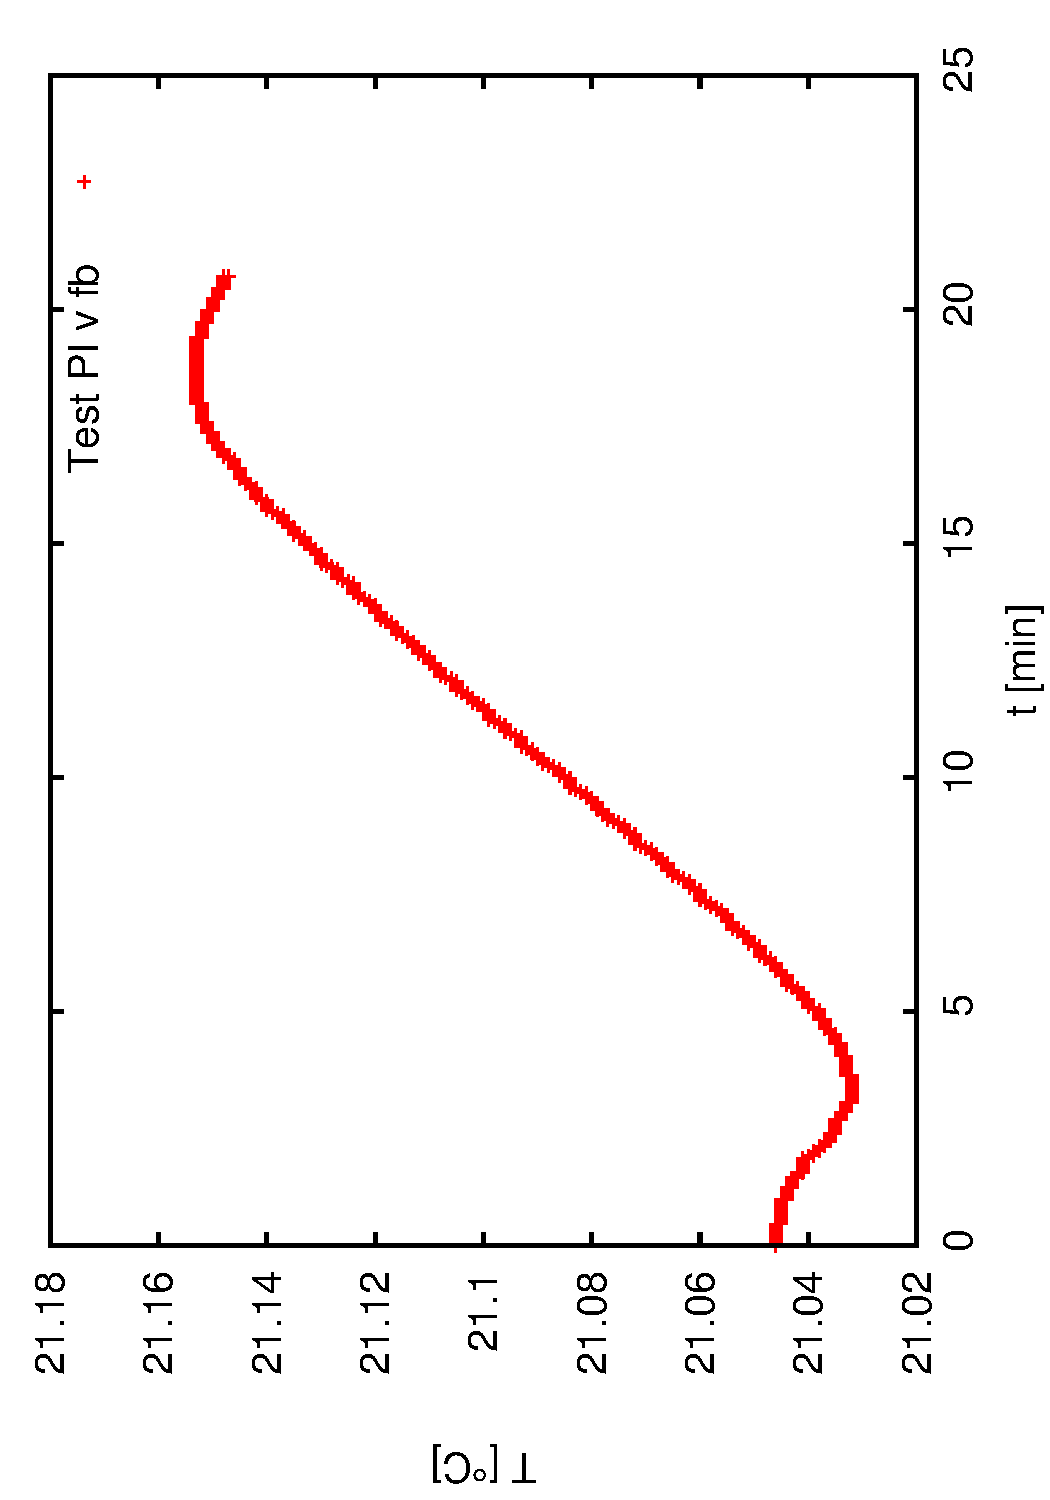
\includegraphics[angle=-90,scale=0.20]{image01a.pdf}\caption{PI movers linearity test without FB (up) and with FB (down). Non linear effect is visible for the movers without FB. Temperature was registered.}\label{f-PIlinearity}
\end{center}
\end{figure}
\begin{figure}
 \begin{center}
 \includegraphics[angle=-90,scale=0.30]{image14.pdf}
 \includegraphics[angle=-90,scale=0.30]{image04.pdf}
 \caption{Settling speed without feedback (left) and with feedback for PI movers.}
% \includegraphics[angle=-90,scale=0.16]{image05c.pdf}
\end{center}
\end{figure}
Each step is 0.1V (3$\mu$m), sampled 15 times (over 3 s). Last 10 points were used to calculate the mean on each step, error over the mean of each step: less than 3nm. System can respond at 3$\mu$m$/$s\par
\begin{figure}
\begin{center}
 \includegraphics[angle=-90,scale=0.50]{image06e.pdf}\caption{Residual non-linearity (with fb), after substraction of linear fitting on PI movers.}\label{f-PIlinres}
\end{center}
\end{figure}
\begin{table}
\begin{center}
\begin{tabular}[]{|c|c|c|}\hline
 Cycle & Slope[nm/V] & Offset[nm] \\\hline
 {\color{red}1} & $-30011 \pm 1$& $-191\pm9$\\
{\color{green}2} & $-29997 \pm 1$& $-204\pm9$ \\
{\color{blue}3} & $-29982 \pm 2$& $-502\pm9$\\
{\color{magenta}4} & $-30018 \pm2$ & $84\pm11$\\\hline
\end{tabular}\caption{Fit result per cycle in PI movers with FB.}\label{t-PIfit}
\end{center}
\end{table}
Slope mean = $30002\pm7\mu$m/V, however, previous result by Frédéric Bogard showed $\sim$120nm/0.1$^\circ$C, if no thermal response delay.
\subsubsection{Cedrat without and with feedback}
Four cycles (two going up, two going down), range (-1$\sim$7V, 0$\sim$250$\mu$m). Each step is 0.1V ($\sim3.125\mu$m), sampled 15 times (over 3 s). Last 10 points were used to calculate the mean on each step\\Error over the mean of each step: less than 15nm. Slope mean = $-31015\pm12$($\pm42$) $\mu$m/V, unknown temperature effect. System can respond at 3$\mu$m$/$s\par
\begin{figure}
\begin{center}
\includegraphics[angle=-90,scale=0.20]{image31.pdf}
\includegraphics[angle=-90,scale=0.20]{image32.pdf}
\includegraphics[angle=-90,scale=0.20]{image31a.pdf}\\
\includegraphics[angle=-90,scale=0.20]{image21.pdf}
\includegraphics[angle=-90,scale=0.20]{image22.pdf}
\includegraphics[angle=-90,scale=0.20]{image21a.pdf}\caption{Cedrat movers linearity test without FB (up) and with FB (down). Non linear effect is visible for the movers without FB. Temperature was registered.}\label{f-Cedratlinearity}
\end{center}
\end{figure}
\begin{figure}
\begin{center}
 \includegraphics[angle=-90,scale=0.30]{image34.pdf}
 \includegraphics[angle=-90,scale=0.30]{image24.pdf}\caption{Settling speed without feedback (left) and with feedback for Cedrat movers.}\label{f-Cedratstep}
%  \includegraphics[angle=-90,scale=0.16]{image25c.pdf}
\end{center}
\end{figure}
\begin{figure}
 \begin{center}
\includegraphics[angle=-90,scale=0.50]{image26e.pdf}\caption{Residual non-linearity (with fb), after substraction of linear fitting on Cedrat movers.}\label{f-Cedratlinres}
\end{center}
\end{figure}
\begin{table}
 \begin{center}
\begin{tabular}[]{|c|c|c|}\hline
 Cycle & Slope[nm/V] & Offset[nm] \\\hline
 {\color{red}1} & $30988 \pm 41$& $-18670\pm154$\\
{\color{green}2} & $31039 \pm 42$& $-19092\pm154$ \\
{\color{blue}3} & $30993\pm 41$& $-18547\pm156$\\
{\color{magenta}4} & $31040 \pm42$ & $-18935\pm154$\\\hline
\end{tabular}\caption{Fit result per cycle in Cedrat movers.}\label{t-Cedratslopes}
\end{center}
\end{table}
\subsubsection{From Gauges}
Lateral fixed
 \includegraphics[angle=-90,scale=0.20]{image_ai_01.pdf}
 \includegraphics[angle=-90,scale=0.20]{image_ai_02.pdf}\\
Verticals fixed
 \includegraphics[angle=-90,scale=0.20]{image_ai_03.pdf}
 \includegraphics[angle=-90,scale=0.20]{image_ai_04.pdf}\\ 

 
 \subsubsection{Summary}
 \;{\tiny Four cycles,range (0$\sim$10V, 0$\sim$300$\mu$m)}\\
\textbf{PI without fb}\hspace*{4cm}\textbf{PI with  fb}\par
\includegraphics[angle=-90,scale=0.10]{image12.pdf}\hspace*{2cm}
\includegraphics[angle=-90,scale=0.10]{image02.pdf}
\includegraphics[angle=-90,scale=0.14]{image06e.pdf}\par
Lateral fixed\hspace{1.8cm}(fb)\hspace{3.0cm}(no fb)\par
 \hspace*{2cm}\includegraphics[angle=-90,scale=0.15]{image_ai_01.pdf}
 \includegraphics[angle=-90,scale=0.15]{image_ai_02.pdf}\\
 Vertical fixed\hspace{1.6cm}(fb)\hspace{3.0cm}(no fb)\\
 \hspace*{2cm}\includegraphics[angle=-90,scale=0.15]{image_ai_03.pdf}
 \includegraphics[angle=-90,scale=0.15]{image_ai_04.pdf}\\
{\tiny Four cycles, range (-1$\sim$7V, 0$\sim$250$\mu$m)}\\
\textbf{Cedrat without fb}\hspace*{3.2cm}\textbf{Cedrat with  fb}\par
\includegraphics[angle=-90,scale=0.10]{image32.pdf}\hspace*{2cm}
\includegraphics[angle=-90,scale=0.10]{image22.pdf}
\includegraphics[angle=-90,scale=0.14]{image26e.pdf}\par
Lateral fixed\hspace{1.8cm}(fb)\hspace{3.0cm}(no fb)\par
 \hspace*{2cm}\includegraphics[angle=-90,scale=0.15]{image_ai_11.pdf}
 \includegraphics[angle=-90,scale=0.15]{image_ai_12.pdf}\\
 Vertical fixed\hspace{1.6cm}(fb)\hspace{3.0cm}(no fb)\\
  \hspace*{2cm}\includegraphics[angle=-90,scale=0.15]{image_ai_13.pdf}
 \includegraphics[angle=-90,scale=0.15]{image_ai_14.pdf}\\ 


\section{Coupling}
\subsection{PI without and with feedback}
Four cycles (two going up, two going down), range (0$\sim$10V, 0$\sim$300$\mu$m)\\
\includegraphics[angle=-90,scale=0.15]{image51.pdf}
\includegraphics[angle=-90,scale=0.15]{image52.pdf}
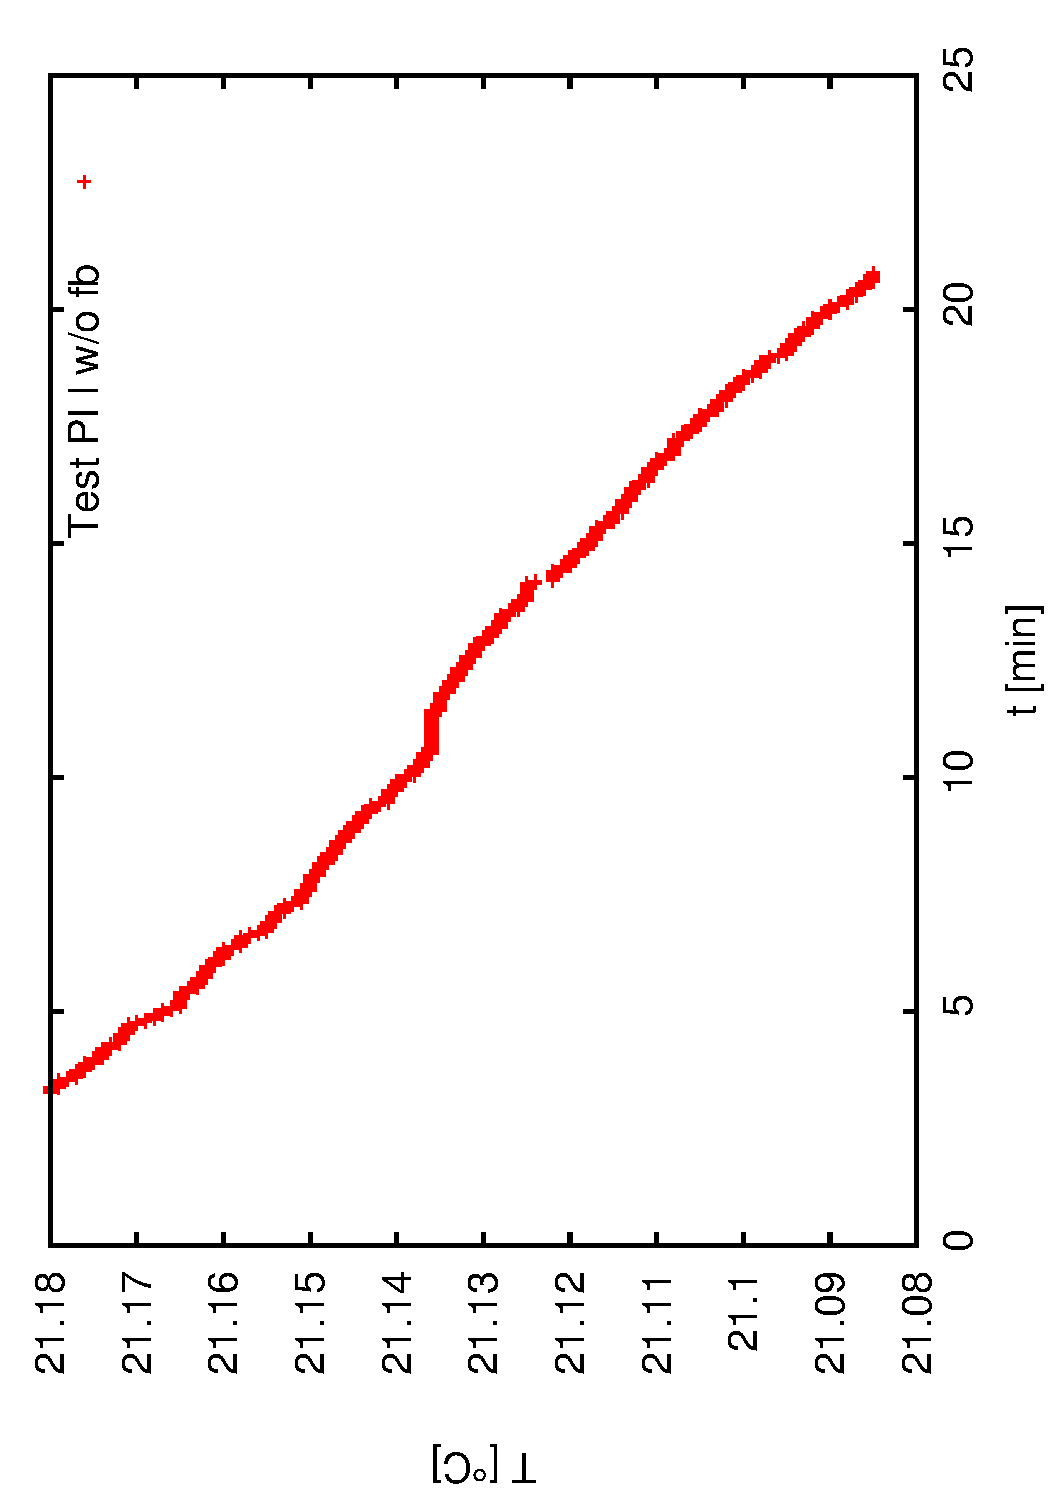
\includegraphics[angle=-90,scale=0.15]{image51a.pdf}\\

\includegraphics[angle=-90,scale=0.15]{image41.pdf}
\includegraphics[angle=-90,scale=0.15]{image42.pdf}
\includegraphics[angle=-90,scale=0.15]{image41a.pdf}\\

\subsubsection{Cedrat without and with feedback}
Four cycles (two going up, two going down), range (-1$\sim$7.0V, 0$\sim$250$\mu$m)\\
\includegraphics[angle=-90,scale=0.15]{image71.pdf}
\includegraphics[angle=-90,scale=0.15]{image72.pdf}
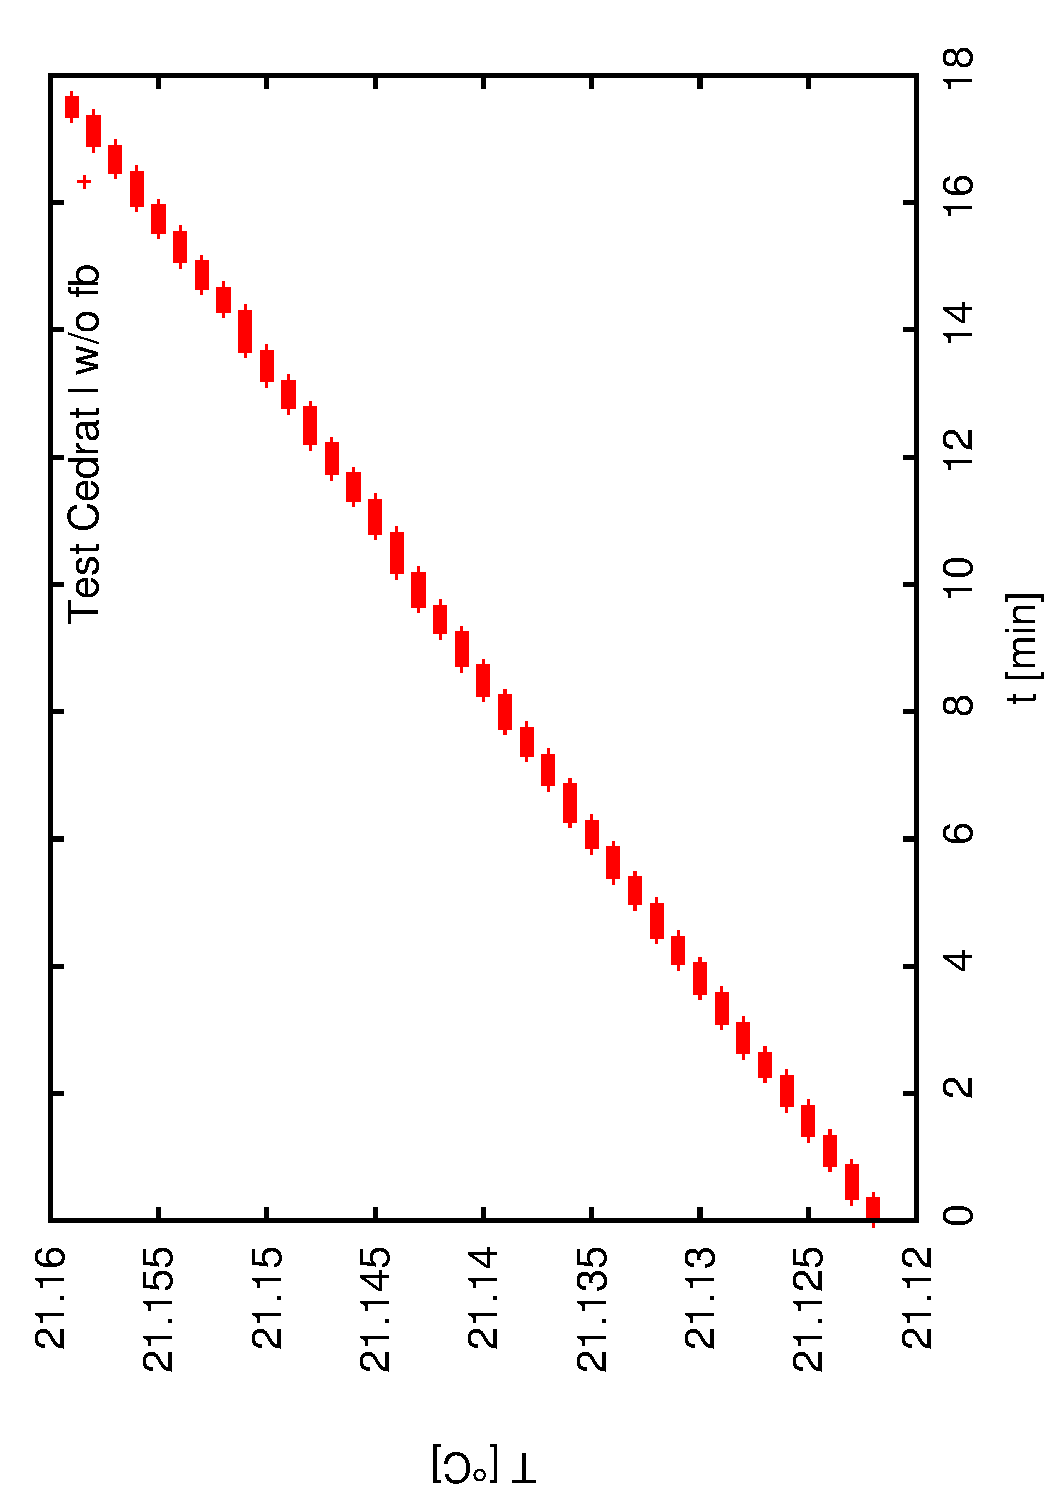
\includegraphics[angle=-90,scale=0.15]{image71a.pdf}\\
\includegraphics[angle=-90,scale=0.15]{image61.pdf}
\includegraphics[angle=-90,scale=0.15]{image62.pdf}
\includegraphics[angle=-90,scale=0.15]{image61a.pdf}\\

\subsubsection{Summary}
\;{\tiny Four cycles, range (0$\sim$10V, 0$\sim$300$\mu$m)}\\
\textbf{PI without fb}\hspace*{2.6cm}\textbf{PI with  fb}\par
\includegraphics[angle=-90,scale=0.10]{image52.pdf}\hspace*{2cm}
\includegraphics[angle=-90,scale=0.10]{image42.pdf}\\
Coupling of $3\mu$m over all lateral range, equivalent to ($1\%$)\\
{\tiny Four cycles, range (-1$\sim$7.0V, 0$\sim$250$\mu$m)}\\
\textbf{Cedrat without fb} \hspace*{1.6cm}\textbf{Cedrat with fb}\par
\includegraphics[angle=-90,scale=0.10]{image72.pdf}\hspace*{2cm}
\includegraphics[angle=-90,scale=0.10]{image62.pdf}\\
Coupling of $2.5\mu$m over all lateral range, equivalent to ($1\%$)\par

\section{Stability and Minimum Step}
\subsection{PI without and with feedback}
\includegraphics[angle=-90,scale=0.20]{imagestep01.pdf}
\includegraphics[angle=-90,scale=0.20]{imagestep01a.pdf}\\
\includegraphics[angle=-90,scale=0.20]{imagestep21.pdf}
\includegraphics[angle=-90,scale=0.20]{imagestep21a.pdf}\\
{\scriptsize 0.5mV$\rightarrow$15nm}\\
\subsection{Cedrat without and with feedback}
\includegraphics[angle=-90,scale=0.20]{imagestep12.pdf}
\includegraphics[angle=-90,scale=0.20]{imagestep12a.pdf}\\
\includegraphics[angle=-90,scale=0.20]{imagestep31.pdf}
\includegraphics[angle=-90,scale=0.20]{imagestep31a.pdf}\\
{\scriptsize 0.5mV$\rightarrow$15.625nm}\\
\subsection{Some vibration}
\includegraphics[angle=-90,scale=0.20]{imagefft02.pdf}
\includegraphics[angle=-90,scale=0.20]{imagefft01.pdf}\\
\subsection{Temperature}
\hspace*{1.2cm}First test (no fb)\hspace{2cm}Second test (fb)\par
 \includegraphics[angle=-90,scale=0.18]{image_ai_31a.pdf}
 \includegraphics[angle=-90,scale=0.18]{image_ai_31b.pdf}\\
 \hspace*{2.5cm}\includegraphics[angle=-90,scale=0.18]{image_ai_31.pdf}\\
\subsection{Some electrical noise}
Stability (PI 1mV$\sim$30nm, Cedrat 1mV$\sim$31.25nm)\par
PI at 5V \hspace{0.5cm}(fb, $\sigma<=1.4$mV$\rightarrow$5.3mV)\hspace{0.4cm}(no fb, $\sigma<=$1.6mV)\par
 \hspace*{2cm}\includegraphics[angle=-90,scale=0.15]{image_ai_21a.pdf}
 \includegraphics[angle=-90,scale=0.15]{image_ai_21.pdf}\\
Cedrat at 3V\hspace{0.4cm}(fb, $\sigma<=0.8$mV)\hspace{1.0cm}(no fb, $\sigma<=0.6$mV)\\
  \hspace*{2cm}\includegraphics[angle=-90,scale=0.15]{image_ai_21c.pdf}
 \includegraphics[angle=-90,scale=0.15]{image_ai_21b.pdf}\\ 
 
 Previous result (stability)\par
 \includegraphics[scale=0.25,angle=0]{image_PI_avant_partir.jpg}\par
Stability (PI 1mV$\sim$30nm, Cedrat 1mV$\sim$31.25nm)\par
PI at 5V \hspace{0.5cm}(fb, $\sigma<=1.4$mV$\rightarrow${\color{red}5.3mV})\hspace{0.4cm}(no fb, $\sigma<=$1.6mV)\par
 \hspace*{2cm}\includegraphics[angle=-90,scale=0.15]{image_ai_21a.pdf}
 \includegraphics[angle=-90,scale=0.15]{image_ai_21.pdf}\\
Cedrat at 3V\hspace{0.4cm}(fb, $\sigma<=0.8$mV)\hspace{1.0cm}(no fb, $\sigma<=0.6$mV)\\
  \hspace*{2cm}\includegraphics[angle=-90,scale=0.15]{image_ai_21c.pdf}
 \includegraphics[angle=-90,scale=0.15]{image_ai_21b.pdf}\\ 
PI Strain Gauges -- Before Installation (1$\sim$2mV)\par
Cedrat Movers are {\color{green}OK}, PI movers have an {\color{red}increase in noise}.
%  \begin{array}{cc}
%  \hspace*{2.3cm}Default Synrad\hspace*{3.3cm}Flag ``-six\_dim 1''\par
%\includegraphics[scale=0.20,angle=-90]{imagestep01.pdf}
\par
After installation\par
PI Strain Gauges -- After Installation\par
 Several test were performed during and after installation\par
 \begin{itemize}
  \item Last day of installation, it seems that noise was initially not present.
  \item After an hour, something change and noise appears abruptly.
  \item After the chamber installation, in order to check if there was a problem with the DACs, gauge cables channels 0 and B were swapped and remote data acquistion was made again obtaining same result.
  \item After shut down and reinitialization ATF period, data was acquired again having same RMS and similar histogram.
 \end{itemize}
 NOTE:
 All test were made setting movers at mid range except most recent one were all was set to zero volts.\par
PI Strain Gauges -- After Installation\par
\centering{\color{red} VERTICAL MOVERS}\\
\hspace*{4.4cm}\textbf{Remotely}\\
\hspace*{0.8cm}Before noise \hspace{1.8cm} First test \hspace{2.0cm}Second test (swap)\par
 \includegraphics[scale=0.15,angle=-90]{image_ai_21e1.pdf}
%  \includegraphics[scale=0.15,angle=-90]{image_ai_21e2.pdf}
  \includegraphics[scale=0.15,angle=-90]{image_ai_23e1.pdf}
  \includegraphics[scale=0.15,angle=-90]{image_ai_24e1.pdf}\par
%  \end{array}
\includegraphics[scale=0.15,angle=-90]{image_ai_21e3.pdf}
%  \includegraphics[scale=0.15,angle=-90]{image_ai_21e4.pdf}
 \includegraphics[scale=0.15,angle=-90]{image_ai_23e3.pdf}
 \includegraphics[scale=0.15,angle=-90]{image_ai_24e3.pdf}\par
\includegraphics[scale=0.15,angle=-90]{image_ai_21e5.pdf}
%  \includegraphics[scale=0.15,angle=-90]{image_ai_21e6.pdf}
 \includegraphics[scale=0.15,angle=-90]{image_ai_23e5.pdf}
 \includegraphics[scale=0.15,angle=-90]{image_ai_24e5.pdf}\par
 \vspace{1cm}
\centering{\color{red} LATERAL MOVER}\\
  \includegraphics[scale=0.15,angle=-90]{image_ai_21e7.pdf}
%  \includegraphics[scale=0.15,angle=-90]{image_ai_21e8.pdf}
 \includegraphics[scale=0.15,angle=-90]{image_ai_23e7.pdf}
 \includegraphics[scale=0.15,angle=-90]{image_ai_24e7.pdf}\par
 
Movers System (cont.)
During tests at LAL\par
\begin{center}
\begin{tikzpicture}
 \node (img1) {\includegraphics[scale=0.5]{Page2.pdf}};
 \node (img2) at (4.4,1.5) {\includegraphics[scale=0.1,angle=-90]{imagestep12.pdf}};
 \node (img3) at (4.4,2.6) {$\sigma_y<2$nm};
\end{tikzpicture}
\end{center}
Noise$<$2mV was measured by the ADCs\\
{\tiny BLOCK AB 1mV=31.25nm, BLOCK C 1mV=30nm}\par
After installation\par
\begin{center}
\begin{tikzpicture}
 \node (img1) {\includegraphics[scale=0.5]{Page1.pdf}};
 \node (img2) at (4.4,1.5) {\includegraphics[scale=0.1,angle=-90]{imagestep12.pdf}};
%  \node (img3) at (4.4,2.6) {$\sigma_y=$?};
 \node (img3) at (4.4,1.5) {{\LARGE\color{red} ?}};
\end{tikzpicture}
\end{center}
Noise about $\sim$2mV was measured by the ADC BLOCK AB\\
\hspace*{2.05cm}{\color{red}$\sim$5mV for BLOCK C} (appears and disappears)\\
{\tiny BLOCK AB 1mV=31.25nm, BLOCK C 1mV=30nm}\par


 \raggedright
\subsubsection{Summary}
\textbf{PI without  fb}\\
\includegraphics[angle=-90,scale=0.15]{imagestep21.pdf}
\includegraphics[angle=-90,scale=0.15]{imagestep21a.pdf}\\
\textbf{PI with  fb}\\
\includegraphics[angle=-90,scale=0.15]{imagestep01.pdf}
\includegraphics[angle=-90,scale=0.15]{imagestep01a.pdf}\\
{\scriptsize 0.5mV$\rightarrow$15nm}\\
% \hspace*{4.3cm}
\textbf{Cedrat without fb}\\
\includegraphics[angle=-90,scale=0.15]{imagestep31.pdf}
\includegraphics[angle=-90,scale=0.15]{imagestep31a.pdf}\\
% \hspace*{4.6cm}
\textbf{Cedrat with fb}\\
\includegraphics[angle=-90,scale=0.15]{imagestep12.pdf}
\includegraphics[angle=-90,scale=0.15]{imagestep12a.pdf}\\
{\scriptsize 0.5mV$\rightarrow$15.625nm}\\

\section{Electrical}
\subsection{GND connection}
 Just one channel was analyzed (PI E)\\
 When GND is {\color{green}disconnected}, additional frequency components were present.\par
\includegraphics[angle=-90,scale=0.30]{image_ai_41.pdf}\\
We chose {\color{blue}GND connected}.\par

\section{Alignment}
\subsection{Previous Vertical Mechanical Alignment Status}
Previous Vertical Mechanical Alignment
\centering\vspace*{0cm}
\textbf{Position referred to {\color{blue} baseplate}}\\
\raggedright
\begin{minipage}{0.5\textwidth}
\begin{tikzpicture}
\draw (0, 0) node[inner sep=0] {\includegraphics[scale=0.2,angle=0]{fig001.jpg}};\\
     \draw (1, 1) node {\hspace*{-5.0cm}\includegraphics[scale=0.15,angle=0]{fig12.pdf}};
\end{tikzpicture}
\end{minipage}\hfill\hspace*{-2cm}\vspace*{2cm}
\begin{minipage}{0.5\textwidth}
Measurements with 3D arm\\
\hspace*{0.5cm}(50$\mu$m precision)\\
Vertical measurements with laser
\hspace*{0.5cm}(1$\mu$m precision)\\
BPM AB Pitch: 1.7mrad\\
BPM C Pitch: -0.5mrad
\end{minipage}\\\vspace*{-1.2cm}
Pitch measured in the external BPM surfaces did not explain the BPM C $Q_y$ signal. Even so, some shims were added to compensate
\begin{table}[htb]
\begin{center}
\begin{tabular}{|l|c|c|c|c|c|c|}\hline
 MOVER & 1&2&3&C&D&E\\\hline\hline
 SHIM [$\mu$m]& 160&165&160&110&110&\\
 &160&155&160&200&205&\\
 &105$^L$&105$^L$&105$^L$&20&20&\\
 &205$\sim$210&205$\sim$210&205&60&50&\\\hline\hline
 TOTAL [$\mu$m]&630$\sim$635&630$\sim$635&630&390&385&\\\hline
 DESIRED[$\mu$m]& 600&600&600&370&370&0\\\hline
\end{tabular}
\caption{Shims installed to compensate beam pitch signal. No mechanical misalignment was found. Columns show the shims installed values and the desired value to correct pitch signal. Each shim width was measured before installation. However, they came in different lateral sizes. Shims marked with $^L$ are larger than the others. Each shim was measured within $\pm5\;\mu$m}
\end{center}
\end{table}




\subsubsection{Block IP-BPMA and IP-BPMB}
Previous Status: \textbf{Pitch}\\
\begin{minipage}{0.5\textwidth}
\begin{tikzpicture}
\draw (0, 0) node[inner sep=0] {\hspace*{0.7cm}\includegraphics[scale=0.22,angle=0]{fig06.pdf}};
\end{tikzpicture}
\end{minipage}\hfill\hspace*{-2cm}\vspace*{2cm}
\begin{minipage}{0.5\textwidth}
Qualitatively\\
@IPBPM-A: $I_y=0, Q_y=0$\\
@IPBPM-B: $I_y=0, Q_y=0$\\
40db attenuation\\
Offset=167.4$\mu$m (5.4V)\\
Angle=1.377mrad=$\arcsin\left(\frac{167.4\mu \text{m}}{121.6\text{mm}}\right)$\\
\hspace*{0.7cm}between movers 3 and 1,2\\
\end{minipage}\\
\vspace*{-2.0cm}
Current Status: \textbf{No pitch, No misalignment}\\
\begin{minipage}{0.5\textwidth}
\begin{tikzpicture}
\draw (0, 0) node[inner sep=0] {\hspace*{0.7cm}\includegraphics[scale=0.22,angle=0]{fig10.pdf}};
\end{tikzpicture}
\end{minipage}\hfill\hspace*{-2cm}
\begin{minipage}{0.5\textwidth}
Qualitatively\\
@IPBPM-A: $I_y=0, Q_y=0$\\
@IPBPM-B: $I_y=0, Q_y=0$\\
Pitch angle = 0\\
(from limited position resolution with 40db att.)
\end{minipage}\\


Block IP-BPMC
Previous Status: \textbf{Pitch}\\
\begin{minipage}{0.5\textwidth}
\begin{tikzpicture}
\draw (0, 0) node[inner sep=0] {\hspace*{0.7cm}\includegraphics[scale=0.22,angle=-45]{fig13.pdf}};
\end{tikzpicture}
\end{minipage}\hfill\hspace*{-2cm}\vspace*{2cm}
\begin{minipage}{0.5\textwidth}
Qualitatively\\
@IPBPM-C: $I_y=0, Q_y\neq0$\\
40db attenuation\\
Movers dynamic range was not enough to compensate the angle.\\
Pitch estimated in 5.7mrad by angle scan $10\beta_y1\beta_x$ optics.
\end{minipage}\\
\vspace*{-2.0cm}
Current Status: \textbf{No pitch}\\
\begin{minipage}{0.5\textwidth}
\begin{tikzpicture}
\draw (0, 0) node[inner sep=0] {\hspace*{0.7cm}\includegraphics[scale=0.22,angle=0]{fig11.pdf}};
\end{tikzpicture}
\end{minipage}\hfill\hspace*{-2cm}
\begin{minipage}{0.5\textwidth}
Qualitatively\\
@IPBPM-C: $I_y=0, Q_y=0$\\
Pitch angle = 0\\
(from limited position resolution with 40db att.)
\end{minipage}\\

\subsection{Current status}
Block AB and C Alignment\par
% \begin{columns}
%  \begin{column}{5cm}
 \includegraphics[scale=0.3,angle=0]{fig20.pdf}\\
{\tiny Using BPMB as reference,  $1000\beta_y$ optics}
%  \end{column}
%  \begin{column}{5cm}
%  \vspace*{-1.0cm}
 \includegraphics[scale=0.3,angle=0]{fig28.pdf}\\
%  \end{column}
% \end{columns}\par\centering
\begin{center}
 \begin{tabular}{|c||c|c|c|}\hline
 &\multicolumn{2}{|c|}{Beam test 1}& Beam test 2\\\cline{2-4}
 & B & A &C\\\hline\hline
$x_0$ [$\mu$m] & $0\pm5$ & $53\pm5$ &$180?\pm?$\\
$y_0$ [$\mu$m]& $0\pm3$ & $\boldsymbol{-34\pm3}$ &$\boldsymbol{-55\pm23}$\\
$z_0$ [mm]& not meas. & not meas. & not meas.\\
$\theta_{p0}$ [mrad]& $0\pm0.1$ & $\boldsymbol{1.6\pm0.1}$ & $\boldsymbol{<1.6}$\\
$\theta_{r0}$ [mrad]& not meas.&not meas.&not meas.\\
$\theta_{y0}$ [mrad]& not meas.&not meas.&not meas.\\\hline
\end{tabular}
\end{center}

% $-1<{\color{magenta} M_{0,1,2,3}}<1,{\color{magenta}\Delta M_{0,1,2,3}}\geq1.25\times 10^{-2}$\par
\subsection{Possible Corrections}
Using BPMB as reference,  $1000\beta_y$ optics\par
\begin{tabular}{|c||c|c|c|}\hline
 &\multicolumn{3}{|c|}{Adjustment (if BPM B is reference and centered)}\\\cline{2-4}
 & B & A & C\\\hline\hline
% $x$[$\mu$m] & ${\color{magenta}125M_0}$ & $53+{\color{magenta}125M_0}$&${180+\color{magenta}150M_{B}}$\\
$y$[$\mu$m]& ${\color{magenta}94.8M_{1,2}+30.2M_3}$ & $-34+{\color{magenta}11.2M_{1,2}+113.8M_3}$&$-55+{\color{magenta}128.0M_{CD}+22.0M_E}$\\
% $z$[mm]& not meas. & not meas.& not meas.\\
$\theta_{p}$[mrad]& ${\color{magenta}1.03(M_3-M_{1,2})}$ & $1.6+{\color{magenta}1.03(M_3-M_{1,2})}$ &$<1.6+{\color{magenta} 2.02(M_{DC}-M_E)}$\\\hline
% $\theta_{r}$[mrad]& not meas.&not meas.&not meas.\\
% $\theta_{y}$[mrad]& not meas.&not meas.&not meas.\\\hline
\end{tabular}\par
Horizontal position seems to be possible to correct.\par
Vertical correction at least to $\mu$m precision is possible between:
\begin{itemize}
 \item A and C
 \item B and C.
\end{itemize}
V:\hspace*{0.1cm} $y_B=\boldsymbol{0\mu}$\textbf{m}, $\theta_{Bp}=\boldsymbol{0}$\textbf{mrad},\hspace{10mm} $y_A=-34\mu$m, $\theta_{Bp}=1.6$mrad\\
\hspace*{0.45cm} $y_B=\boldsymbol{0\mu}$\textbf{m}, $\theta_{Bp}=0.4$mrad,\hspace{7mm} $y_A=\boldsymbol{0\mu}$\textbf{m	}, $\theta_{Bp}=2.0$mrad\\
\hspace*{0.45cm} $y_B=0\mu$m, $\theta_{Bp}=\boldsymbol{-0.8}$\textbf{mrad},\hspace{3mm} $y_A=-64.9\mu$m, $\theta_{Bp}=\boldsymbol{0.8}$\textbf{mrad}\\
\hspace*{0.45cm} $y_B=21.9\mu$m, $\theta_{Bp}=-1.6$mrad, $y_A=-107.64\mu$m, $\theta_{Bp}=\boldsymbol{0}$\textbf{mrad}\\